\section{Absorption models and the method of characteristics}
\label{sec:moc}

The models considered so far describe the population inside a single compartment.
Once several compartments share a medium, a further question arises: what becomes
of the contents of the first compartment to rupture? The shared medium acquires, at
a stroke, a potentially large cohort of particles available for subsequent
absorption by the compartments that remain.

The analysis to this point has assumed \emph{immediate transfer}, in which the
entire contents of a ruptured compartment relocate at once into the interior of
another. That is a strong assumption. The alternative is an \emph{absorption
period}: following a rupture, absorption events redistribute the released cohort
among the remaining compartments, and only when every particle has been taken up do
birth, death and rupture resume. Working towards models of that kind, this section
treats the case in which a cohort of particles enters a single compartment.

Three models are treated in increasing order of difficulty. In the first two the
particles are conserved or only lost, the state space is finite, and an
independence argument delivers the generating function with no need to solve a
partial differential equation at all. In the third, replication inside the
compartment opens an infinite state space and the independence shortcut fails, so
the equation must be confronted directly. The method of characteristics is
therefore developed on the second model, where the answer is already known, and
then applied to the third. The closed form obtained for the third model,
\cref{prop:Gabd}, is a result of this thesis.

\subsection{Absorption only}
\label{sec:absonly}

The simplest absorption process has a single compartment that takes in particles,
with no subsequent dynamics: no birth and no death within the compartment.

Let $X_t$ and $Y_t$ count the particles inside and outside the compartment
respectively; the same labelling is used for every version of the
single-compartment model below. Events are stochastic with exponentially
distributed inter-event times, which by \cref{sec:exp} follows from the assumption
that event rates do not depend on time, so that $\{(X_t,Y_t):t\ge0\}$ is a
continuous-time Markov chain in the sense of \cref{sec:ctmc}.

With only absorption to consider, the model is specified by the transition
probabilities over an infinitesimal interval $\Delta t$,
\begin{align*}
\pr{\Delta X = 1,\ \Delta Y = -1 \mid Y_t = j} &= j\alpha\,\Delta t, &&\text{(absorption)}\\
\pr{\Delta X = 0,\ \Delta Y = 0 \mid Y_t = j} &= 1-j\alpha\,\Delta t, &&\text{(no event)}
\end{align*}
where $\Delta X = X_{t+\Delta t}-X_t$ and similarly for $Y$, and terms of
$o(\Delta t)$ are suppressed throughout. The factor $j$ records that each exterior
particle is independently subject to the same probability $\alpha\Delta t$ of being
taken up. The initial condition is $X_0=0$, $Y_0=N$: a starter population of $N$
particles occupying the exterior medium.

Writing $p_{i,j}(t) = \pr{X_t=i,\ Y_t=j}$, the forward Kolmogorov equations are
\begin{equation}
\label{eq:FK1}
\ddt{p_{i,j}} = \alpha(j+1)p_{i-1,j+1} - \alpha j\,p_{i,j} .
\end{equation}
With the bivariate generating function
\begin{equation}
\label{eq:pgfDef}
G(x,y,t) = \sum_i\sum_j p_{i,j}(t)\,x^iy^j = \ex{x^{X_t}y^{Y_t}},
\end{equation}
\cref{eq:FK1} converts into a partial differential equation by the procedure of
\cref{sec:pgf}. Multiply each equation by $x^iy^j$ and sum over $i$ and $j$; the
sums are finite, because $p_{i,j}(t)=0$ whenever $i+j\neq N$, particles in this
model being neither created nor destroyed. Shifting indices in the first term
sends $\alpha(j+1)p_{i-1,j+1}x^iy^j$ to $\alpha x\,\partial_yG$, and the second
term is $-\alpha y\,\partial_yG$, so that
\begin{equation}
\label{eq:PDE1}
\pddt{G} = \alpha(x-y)\pdd{G}{y},
\qquad G(x,y,0) = y^N .
\end{equation}

This first-order linear initial value problem is more awkward than it looks. The
method of characteristics applies in principle to equations in three variables, but
applying it here is not straightforward, and it is postponed to
\cref{sec:mocabsdeath}. The solution can be obtained by other means, and it is
worth doing so both because the answer is needed and because it provides a check on
the machinery developed there.

\subsubsection*{Exploiting independence}

The function $G$ above was specific to $X_0=0$, $Y_0=N$. Define more generally
\begin{equation*}
G_n(x,y,t) = \sum_i\sum_j\pr{X_t=i,\ Y_t=j \mid X_0=0,\ Y_0=n}\,x^iy^j .
\end{equation*}
In a process of pure absorption the $n$ particles are taken up one by one, and the
behaviour of any one of them does not depend on the movements of its neighbours.
That independence lets $X_t$ and $Y_t$ decompose into sums of $n$ single-particle
variables,
\begin{equation*}
X_t = \sum_{k=1}^{n}X_t^{(k)},
\qquad
Y_t = \sum_{k=1}^{n}Y_t^{(k)},
\end{equation*}
from which
\begin{equation}
\label{eq:indRelPGF}
G_n(x,y,t) = \bigl(G_1(x,y,t)\bigr)^n ,
\end{equation}
since
\begin{equation*}
G_n(x,y,t)
= \ex{\prod_{k=1}^{n}x^{X_t^{(k)}}\prod_{k=1}^{n}y^{Y_t^{(k)}}}
= \prod_{k=1}^{n}\ex{x^{X_t^{(k)}}y^{Y_t^{(k)}}}
= \bigl(G_1(x,y,t)\bigr)^n .
\end{equation*}

Now consider a single initial particle, $X_0=0$, $Y_0=1$. It is eventually
absorbed, and that is the final state of the system: no other states are reachable,
so $p_{i,j}(t)=0$ whenever $i+j\neq1$. The forward equations reduce to
\begin{equation*}
\ddt{p_{0,1}} = -\alpha p_{0,1},
\qquad
\ddt{p_{1,0}} = \alpha p_{0,1},
\end{equation*}
giving $p_{0,1}(t) = \ee^{-\alpha t}$ and $p_{1,0}(t) = 1-\ee^{-\alpha t}$
(\cref{fig:abs1}). These being the only two non-zero state probabilities of the
single-particle system,
\begin{equation*}
G_1(x,y,t) = p_{1,0}(t)\,x + p_{0,1}(t)\,y
= \lrb{1-\ee^{-\alpha t}}x + \ee^{-\alpha t}y ,
\end{equation*}
and \cref{eq:indRelPGF} gives the generating function for any initial census,
\begin{equation}
\label{eq:Gabsonly}
G_n(x,y,t) = \Bigl(\lrb{1-\ee^{-\alpha t}}x + \ee^{-\alpha t}y\Bigr)^n .
\end{equation}
This satisfies \cref{eq:PDE1} together with the initial condition
$G_n(x,y,0)=y^n$. The form is recognisable: $X_t\sim\text{Binomial}(n,1-\ee^{-\alpha t})$,
as it must be, since the $n$ particles are absorbed independently and each has been
taken up by time $t$ with probability $1-\ee^{-\alpha t}$.

\begin{figure}[H]
\centering
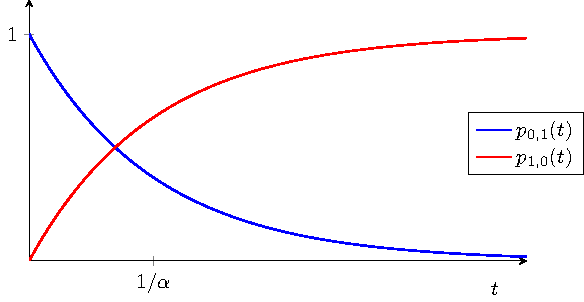
\includegraphics[width=0.62\textwidth]{figures/IMG_ch3/abs1.pdf}
\caption{State probabilities for the single-particle absorption-only model. The
particle begins outside the compartment ($p_{0,1}$, decaying exponentially at rate
$\alpha$) and ends inside it ($p_{1,0}$). There is nowhere else for it to go, so
the two curves sum to one at every time.}
\label{fig:abs1}
\end{figure}

\subsection{Absorption--death}
\label{sec:absdeath}

A particle resident in a compartment may die. Keeping $X_t$ and $Y_t$ for the
interior and exterior counts, death enters as follows:
\begin{align*}
\pr{\Delta X = 1,\ \Delta Y = -1 \mid Y_t=j} &= j\alpha\,\Delta t, &&\text{(absorption)}\\
\pr{\Delta X = -1,\ \Delta Y = 0 \mid X_t=i} &= i\mu\,\Delta t, &&\text{(death)}\\
\pr{\Delta X = 0,\ \Delta Y = 0 \mid X_t=i,\ Y_t=j} &= 1-(j\alpha+i\mu)\Delta t, &&\text{(no event)}
\end{align*}
with forward Kolmogorov equations
\begin{equation}
\label{eq:FK2}
\ddt{p_{i,j}} = \alpha(j+1)p_{i-1,j+1} + \mu(i+1)p_{i+1,j} - (\alpha j+\mu i)p_{i,j} .
\end{equation}
The derivation of \cref{sec:absonly} carries over unchanged and gives the
first-order linear equation
\begin{equation}
\label{eq:PDE2}
\pddt{G} = \mu(1-x)\pdd{G}{x} + \alpha(x-y)\pdd{G}{y},
\qquad G(x,y,0) = y^N ,
\end{equation}
and the same difficulty. Once again the solution can be constructed via
\cref{eq:indRelPGF}, since individual particles remain independent.

Without birth events the number of particles cannot exceed its initial value, so
for an isolated particle the generating function has just three terms,
\begin{equation*}
G_1(x,y,t) = p_{0,0}(t) + p_{1,0}(t)\,x + p_{0,1}(t)\,y .
\end{equation*}
The state probabilities follow from
\begin{equation*}
\ddt{p_{0,1}} = -\alpha p_{0,1},
\qquad
\ddt{p_{1,0}} = \alpha p_{0,1} - \mu p_{1,0},
\end{equation*}
whence
\begin{equation}
\label{eq:absdeathstates}
p_{0,1}(t) = \ee^{-\alpha t},
\qquad
p_{1,0}(t) = \frac{\alpha}{\mu-\alpha}\lrb{\ee^{-\alpha t}-\ee^{-\mu t}},
\qquad
p_{0,0}(t) = 1-p_{0,1}(t)-p_{1,0}(t),
\end{equation}
plotted in \cref{fig:abs2}. Applying \cref{eq:indRelPGF} gives the general
generating function
\begin{equation}
\label{eq:Gabsdeath}
G_n(x,y,t) = \Bigl(
1-\tfrac{\mu}{\mu-\alpha}\ee^{-\alpha t} + \tfrac{\alpha}{\mu-\alpha}\ee^{-\mu t}
+ \tfrac{\alpha}{\mu-\alpha}\bigl(\ee^{-\alpha t}-\ee^{-\mu t}\bigr)x
+ \ee^{-\alpha t}y\Bigr)^n .
\end{equation}

\begin{figure}[H]
\centering
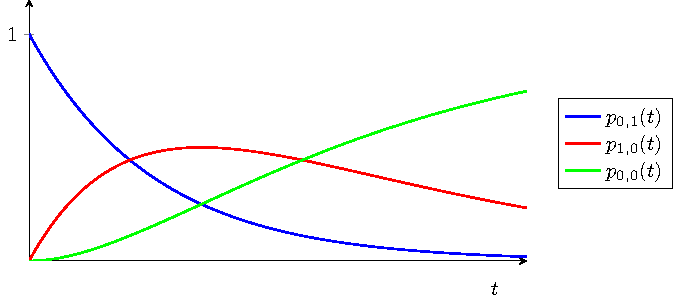
\includegraphics[width=0.62\textwidth]{figures/IMG_ch3/abs2.pdf}
\caption{State probabilities for the single-particle absorption--death model,
\cref{eq:absdeathstates}. The particle starts outside ($p_{0,1}$, blue), is
absorbed into the compartment ($p_{1,0}$, red, which rises and then decays as death
takes over), and finally dies ($p_{0,0}$, green, absorbing).}
\label{fig:abs2}
\end{figure}

\subsection{The method of characteristics, tested on absorption--death}
\label{sec:mocabsdeath}

Before continuing to absorption--birth--death, where replication may occur inside
the compartment and the independence shortcut is unavailable, it is worth
revisiting absorption--death from the point of view of its partial differential
equation. Having \cref{eq:Gabsdeath} already in hand makes it an ideal test
case.\footnote{I am grateful to Benjamin Sharp for the advice on applying the
method of characteristics to three-variate problems that unlocked this section.}

Introduce a change of variables $(x,y,t)\to(\sigma,\eta,\tau)$, writing
\begin{equation*}
G(x,y,t) = G\bigl(x(\sigma,\eta,\tau),\,y(\sigma,\eta,\tau),\,t(\sigma,\eta,\tau)\bigr)
\equiv G(\sigma,\eta,\tau).
\end{equation*}
The method seeks solutions along the characteristic curves of constant $\sigma$ and
$\eta$, on which $G$ is a function of $\tau$ alone. To fix the parametrisation we
impose an initial surface,
\begin{equation}
\label{eq:ICpar}
x(\sigma,\eta,0) = \sigma,
\qquad
y(\sigma,\eta,0) = \eta,
\qquad
t(\sigma,\eta,0) = 0 .
\end{equation}
With $G$ a function of $\tau$ only along a characteristic, the chain rule gives
\begin{equation*}
\dda{G}{\tau} = \pddt{G}\dda{t}{\tau} + \pdd{G}{x}\dda{x}{\tau} + \pdd{G}{y}\dda{y}{\tau},
\end{equation*}
which is to be compared with \cref{eq:PDE2} written as
\begin{equation*}
0 = -\pddt{G} + \mu(1-x)\pdd{G}{x} + \alpha(x-y)\pdd{G}{y} .
\end{equation*}
Comparing coefficients yields the characteristic system
\begin{align}
\dda{G}{\tau} &= 0, \label{eq:ch11}\\
\dda{t}{\tau} &= -1, \label{eq:ch12}\\
\dda{x}{\tau} &= \mu(1-x), \label{eq:ch13}\\
\dda{y}{\tau} &= \alpha(x-y). \label{eq:ch14}
\end{align}

\paragraph{The equation for $G$, \eqref{eq:ch11}.}
$G$ is constant along characteristics, so $G$ is a function of $(\sigma,\eta)$
alone. Under \cref{eq:ICpar} the initial condition $G(x,y,0)=y^N$ becomes
$G(\sigma,\eta,0)=\eta^N$, so
\begin{equation}
\label{eq:GetaN}
G(\sigma,\eta,\tau) = \eta^N .
\end{equation}
The whole problem thus reduces to expressing $\eta$ in terms of $(x,y,t)$.

\paragraph{The equation for $t$, \eqref{eq:ch12}.}
Integrating gives $t = -\tau + c(\sigma,\eta)$, and \cref{eq:ICpar} fixes $c=0$:
\begin{equation}
\label{eq:minustau}
t = -\tau .
\end{equation}
The characteristic parameter runs backwards in time, which is what allows the
initial surface to be reached from any $(x,y,t)$.

\paragraph{The equation for $x$, \eqref{eq:ch13}.}
Separating variables gives $1-x = c(\sigma,\eta)\ee^{-\mu\tau}$, and
\cref{eq:ICpar} gives $c = 1-\sigma$:
\begin{equation}
\label{eq:sandxwithtau}
1-x = (1-\sigma)\ee^{-\mu\tau} .
\end{equation}

\paragraph{The equation for $y$, \eqref{eq:ch14}.}
Substituting \cref{eq:sandxwithtau},
\begin{equation*}
\dda{y}{\tau} = \alpha\bigl(1-(1-\sigma)\ee^{-\mu\tau}-y\bigr),
\end{equation*}
and solving with integrating factor $\ee^{\alpha\tau}$,
\begin{equation*}
y = 1-\frac{\alpha}{\alpha-\mu}(1-\sigma)\ee^{-\mu\tau} + c(\sigma,\eta)\ee^{-\alpha\tau} .
\end{equation*}
Applying \cref{eq:ICpar} gives
$c(\sigma,\eta) = \eta + \frac{\alpha}{\alpha-\mu}(1-\sigma)-1$, so
\begin{equation}
\label{eq:ywitheta}
y = 1-\frac{\alpha}{\alpha-\mu}(1-\sigma)\ee^{-\mu\tau}
+ \lrb{\eta + \frac{\alpha}{\alpha-\mu}(1-\sigma)-1}\ee^{-\alpha\tau} .
\end{equation}

\paragraph{Recovering the solution.}
Rearranging \cref{eq:ywitheta} for $\eta$, substituting $\sigma$ from
\cref{eq:sandxwithtau} and $\tau=-t$ from \cref{eq:minustau}, gives
\begin{equation*}
\eta = 1-\frac{\mu}{\mu-\alpha}\ee^{-\alpha t} + \frac{\alpha}{\mu-\alpha}\ee^{-\mu t}
+ \frac{\alpha}{\mu-\alpha}\bigl(\ee^{-\alpha t}-\ee^{-\mu t}\bigr)x
+ \ee^{-\alpha t}y ,
\end{equation*}
and \cref{eq:GetaN} then reproduces \cref{eq:Gabsdeath} exactly. The two routes
agree, and the machinery is ready for the case in which only one of them is
available.

\subsection{Absorption--birth--death}
\label{sec:absbirthdeath}

Introducing replication for particles inside the compartment, the independence
property is still present but no longer serves as a shortcut: from a single initial
particle, birth events make infinitely many states reachable, so $G_1(x,y,t)$ is an
infinite sum and there is nothing to be gained by factorising. The partial
differential equation must therefore be solved directly, and by now that can be
done.

With $X_t$ and $Y_t$ as before, birth at per-capita rate $\lambda$ is added to the
transition probabilities:
\begin{align*}
\pr{\Delta X = 1,\ \Delta Y = -1 \mid Y_t=j} &= j\alpha\,\Delta t, &&\text{(absorption)}\\
\pr{\Delta X = 1,\ \Delta Y = 0 \mid X_t=i} &= i\lambda\,\Delta t, &&\text{(birth)}\\
\pr{\Delta X = -1,\ \Delta Y = 0 \mid X_t=i} &= i\mu\,\Delta t, &&\text{(death)}\\
\pr{\Delta X = 0,\ \Delta Y = 0 \mid X_t=i,\ Y_t=j} &= 1-(j\alpha+i\mu+i\lambda)\Delta t, &&\text{(no event)}
\end{align*}
with forward Kolmogorov equation
\begin{equation}
\label{eq:FK3}
\ddt{p_{i,j}} = \alpha(j+1)p_{i-1,j+1} + \mu(i+1)p_{i+1,j} + \lambda(i-1)p_{i-1,j}
- (\alpha j+\mu i+\lambda i)p_{i,j} .
\end{equation}
The same reasoning as before gives the generating-function equation
\begin{equation}
\label{eq:PDE3}
\pddt{G} = \bigl(\mu-(\mu+\lambda)x+\lambda x^2\bigr)\pdd{G}{x} + \alpha(x-y)\pdd{G}{y},
\qquad G(x,y,0)=y^N ,
\end{equation}
whose $x$-coefficient is exactly the quadratic met in \cref{eq:bdpde} for the
linear birth--death process. Reparametrising $(x,y,t)\to(\sigma,\eta,\tau)$ as in
\cref{sec:mocabsdeath} gives the characteristic system
\begin{align}
\dda{G}{\tau} &= 0, \label{eq:ch21}\\
\dda{t}{\tau} &= -1, \label{eq:ch22}\\
\dda{x}{\tau} &= \mu-(\mu+\lambda)x+\lambda x^2, \label{eq:ch23}\\
\dda{y}{\tau} &= \alpha(x-y), \label{eq:ch24}
\end{align}
with the same initial conditions \cref{eq:ICpar}.

\paragraph{The equations for $G$ and $t$, \eqref{eq:ch21}--\eqref{eq:ch22}.}
As before,
\begin{equation}
\label{eq:GetaN2}
G(\sigma,\eta,\tau) = \eta^N,
\qquad
t = -\tau .
\end{equation}

\paragraph{The equation for $x$, \eqref{eq:ch23}.}
This is a Riccati equation of the same shape as the one governing the survival
probability in \cref{sec:riccati}. Its right-hand side factorises, and the roots
are elementary rather than the surd expression that mechanical use of the quadratic
formula suggests:
\begin{equation}
\label{eq:xpm}
\mu-(\mu+\lambda)x+\lambda x^2 = \lambda(x-x_+)(x-x_-),
\qquad
x_+ = 1,\quad x_- = \frac{\mu}{\lambda} .
\end{equation}
The discriminant is
$\bigl(\tfrac{\mu+\lambda}{2\lambda}\bigr)^2 - \tfrac{\mu}{\lambda}
= \bigl(\tfrac{\lambda-\mu}{2\lambda}\bigr)^2$, a perfect square, so the surds
cancel. It is convenient to name the combination that appears throughout,
\begin{equation}
\label{eq:b1}
b_1 = \lambda(x_+-x_-) = \lambda-\mu ,
\end{equation}
the net interior growth rate. Separating variables in \cref{eq:ch23} and applying
\cref{eq:ICpar} gives the characteristic in the compact form
\begin{equation}
\label{eq:xratio}
\frac{x-x_+}{x-x_-} = \lrb{\frac{\sigma-x_+}{\sigma-x_-}}\ee^{b_1\tau},
\end{equation}
or, solved for $x$,
\begin{equation}
\label{eq:xabd}
x(\tau) = \frac{x_+(\sigma-x_-) - x_-(\sigma-x_+)\ee^{b_1\tau}}
{(\sigma-x_-) - (\sigma-x_+)\ee^{b_1\tau}} .
\end{equation}

\paragraph{The equation for $y$, \eqref{eq:ch24}.}
The last characteristic equation is $\dd y/\dd\tau = \alpha(x-y)$, which with an
integrating factor becomes
\begin{equation}
\label{eq:yint}
\dda{}{\tau}\lrb{\ee^{\alpha\tau}y} = \alpha\,\ee^{\alpha\tau}x(\tau) .
\end{equation}
The integral on the right is where the difficulty lies. Rather than substitute
\cref{eq:xabd} and split the resulting quotient --- which leads to two
hypergeometric integrals and a good deal of bookkeeping --- it is cleaner to expand
$x(\tau)$ first. Writing $x-x_- = (x-x_+)+(x_+-x_-)$ in \cref{eq:xratio} and
solving for $x$ gives
\begin{equation}
\label{eq:xgeom}
x(\tau) = x_+ + (x_+-x_-)\frac{\zeta(\tau)}{1-\zeta(\tau)},
\qquad
\zeta(\tau) = \lrb{\frac{\sigma-x_+}{\sigma-x_-}}\ee^{b_1\tau},
\end{equation}
so that, for $|\zeta|<1$,
\begin{equation*}
x(\tau) = x_+ + (x_+-x_-)\sum_{n=1}^{\infty}\zeta(\tau)^n .
\end{equation*}
Every term is now a pure exponential in $\tau$ and integrates immediately. Writing
$Z = (\sigma-x_+)/(\sigma-x_-)$, so that $\zeta(\tau) = Z\ee^{b_1\tau}$ and
$Z^n\ee^{nb_1\tau} = \zeta^n$,
\begin{align*}
\alpha\int\ee^{\alpha\tau}x(\tau)\,\dd\tau
&= \alpha x_+\!\int\!\ee^{\alpha\tau}\dd\tau
 + \alpha(x_+-x_-)\sum_{n=1}^{\infty}Z^n\!\int\!\ee^{(\alpha+nb_1)\tau}\dd\tau\\
&= \ee^{\alpha\tau}\lrbs{x_+ + \alpha(x_+-x_-)\sum_{n=1}^{\infty}\frac{\zeta^n}{\alpha+nb_1}}
 + \text{const} .
\end{align*}
Setting $\delta = \alpha/b_1$ and using $\alpha(x_+-x_-)/b_1 = \alpha/\lambda$ by
\cref{eq:b1}, this defines the function that carries the whole solution:
\begin{equation}
\label{eq:Psidef}
\Psi(\zeta) = x_+ + \frac{\alpha}{\lambda}\sum_{n=1}^{\infty}\frac{\zeta^{\,n}}{n+\delta},
\qquad
\delta = \frac{\alpha}{b_1} = \frac{\alpha}{\lambda-\mu} .
\end{equation}
So $\alpha\int\ee^{\alpha\tau}x(\tau)\dd\tau = \ee^{\alpha\tau}\Psi(\zeta(\tau)) + \text{const}$,
and integrating \cref{eq:yint} gives
$\ee^{\alpha\tau}y = \ee^{\alpha\tau}\Psi(\zeta(\tau)) + \text{const}$. The initial
condition $y(\sigma,\eta,0)=\eta$, at which $\zeta(0)=Z$, fixes the constant as
$\eta-\Psi(Z)$, so
\begin{equation}
\label{eq:etasolved}
\eta = \ee^{\alpha\tau}\Bigl[y-\Psi\bigl(\zeta(\tau)\bigr)\Bigr] + \Psi(Z) .
\end{equation}
Finally, put $\tau=-t$ and use \cref{eq:xratio}: writing
\begin{equation*}
W = \frac{x-x_+}{x-x_-}
\end{equation*}
we have $\zeta(\tau) = W$ and $Z = W\ee^{-b_1\tau} = W\ee^{b_1t}$. Substituting into
\cref{eq:etasolved} and applying \cref{eq:GetaN2} gives the solution.

\begin{proposition}[Generating function for absorption--birth--death]
\label{prop:Gabd}
With $x_+=1$, $x_-=\mu/\lambda$, $b_1 = \lambda-\mu$, $\delta = \alpha/b_1$,
$W = (x-x_+)/(x-x_-)$ and $\Psi$ as in \cref{eq:Psidef},
\begin{equation}
\label{eq:Gabd}
\boxed{\;
G(x,y,t) = \Bigl\{\ee^{-\alpha t}\bigl[y-\Psi(W)\bigr] + \Psi\bigl(W\ee^{b_1t}\bigr)\Bigr\}^{N}. \;}
\end{equation}
\end{proposition}

Three checks confirm the result. At $t=0$ the two $\Psi$ terms cancel and $G=y^N$,
the required initial condition. At $x=y=1$ we have $W=0$ and $\Psi(0)=x_+=1$, so
$G=1$ and probability is conserved. And setting $x=1$ alone gives
\begin{equation*}
G(1,y,t) = \bigl(\ee^{-\alpha t}y + 1-\ee^{-\alpha t}\bigr)^N,
\end{equation*}
so $Y_t\sim\text{Binomial}(N,\ee^{-\alpha t})$ --- exactly right, since the
exterior particles are absorbed independently at rate $\alpha$ and what happens
inside the compartment cannot affect them. Beyond these, \cref{eq:Gabd} has been
verified numerically against direct integration of the master equation
\cref{eq:FK3}, agreeing to around $10^{-13}$ across sub- and supercritical interior
regimes and for $N=1,2,3$.

\subsubsection*{Hypergeometric form}

The series in \cref{eq:Psidef} is a Gauss hypergeometric function in disguise. With
\begin{equation}
\label{eq:2F1def}
{}_2F_1(a,b;c;z) = \sum_{n=0}^{\infty}\frac{(a)_n(b)_n}{(c)_n}\frac{z^n}{n!},
\qquad
(q)_n = \begin{cases}1, & n=0,\\ q(q+1)\cdots(q+n-1), & n\ge1,\end{cases}
\end{equation}
where $(q)_n$ is the rising Pochhammer symbol \cite{Olver2010}, the case $a=1$,
$b=\delta$, $c=\delta+1$ collapses to a single ratio. Since $(1)_n = n!$ and
\begin{equation}
\label{eq:pochcancel}
\frac{(\delta)_n}{(\delta+1)_n}
= \frac{\delta(\delta+1)\cdots(\delta+n-1)}{(\delta+1)\cdots(\delta+n-1)(\delta+n)}
= \frac{\delta}{\delta+n},
\end{equation}
we have
\begin{equation}
\label{eq:2F1simple}
{}_2F_1(1,\delta;\delta+1;z) = \sum_{n=0}^{\infty}\frac{\delta}{\delta+n}z^n .
\end{equation}
Comparing with \cref{eq:Psidef} and using
$\alpha/(\lambda\delta) = b_1/\lambda = x_+-x_-$,
\begin{equation}
\label{eq:Psihyp}
\Psi(\zeta) = x_+ + (x_+-x_-)\Bigl[{}_2F_1(1,\delta;\delta+1;\zeta)-1\Bigr] .
\end{equation}
\Cref{eq:Gabd} together with \cref{eq:Psihyp} is the closed form. It is not pretty,
but it is a genuine closed form in terms of a standard special function, and the
elementary series \cref{eq:Psidef} is what one would actually evaluate. An
alternative derivation of the same object, by way of the integral
$\int\ee^{h\tau}/(P+Q\ee^{k\tau})\,\dd\tau$, is given in \cref{app:hyp}; that route
is longer, but it produces a general identity of independent use.

\begin{remark}[Domain of validity]
\label{rem:domain}
The series \cref{eq:Psidef} converges for $|\zeta|<1$, and the arguments appearing
in \cref{eq:Gabd} are $W$ and $W\ee^{b_1t}$. In the subcritical interior regime
$\mu>\lambda$ we have $b_1<0$ and $x_- = \mu/\lambda>1$, so for $x\in[0,1]$ the
argument $W$ lies in $[0,\lambda/\mu]\subset[0,1)$ and $W\ee^{b_1t}$ is smaller
still: the series representation is valid on the whole of the unit square, which is
the case of most interest here. When $\lambda>\mu$ the series converges only for
$x$ above the smaller fixed point $\mu/\lambda$, and elsewhere one must use the
analytic continuation of ${}_2F_1$ --- conveniently, the Euler integral
\begin{equation*}
{}_2F_1(1,\delta;\delta+1;\zeta) = \delta\int_0^1\frac{u^{\delta-1}}{1-\zeta u}\,\dd u
\qquad(\delta>0,\ \zeta\notin[1,\infty)),
\end{equation*}
which was used for the numerical verification quoted above.
\end{remark}

\begin{remark}[Resonance]
\label{rem:resonance}
The denominators in \cref{eq:Psidef} vanish when $n+\delta=0$ for some integer
$n\ge1$, that is when
\begin{equation*}
\alpha = n(\mu-\lambda),\qquad n=1,2,\dots
\end{equation*}
This is the classical resonance condition for linearising the $y$-equation: the
decay rate $\alpha$ of the absorption channel coincides with a harmonic of the
interior relaxation rate $\mu-\lambda$. The generating function itself is perfectly
regular there, being analytic in all parameters, so the singularity is removable,
and at resonance the corresponding term acquires a factor $\tau$ --- a secular term
--- in place of the simple exponential. The resonant parameter values form a set of
measure zero and the limit may be taken numerically, but the degeneracy should be
kept in mind when $\alpha$ happens to sit near an integer multiple of $\mu-\lambda$.
\end{remark}

\FloatBarrier
